\documentclass[a5paper, 10pt]{article}

% Текст
\usepackage{listings}
\usepackage[utf8]{inputenc} % UTF-8 кодировка
\usepackage[russian]{babel} % Русский язык
\usepackage{indentfirst} % красная строка в первом параграфе в главе
\renewcommand{\lstlistingname}{Листинг}
% Отображение страниц
\usepackage{geometry} % размеры листа и отступов
\geometry{
	left=12mm,
	top=25mm,
	right=15mm,
	bottom=17mm,
	marginparsep=0mm,
	marginparwidth=0mm,
	headheight=10mm,
	headsep=7mm,
	nofoot}
\usepackage{afterpage,fancyhdr} % настройка колонтитулов
\pagestyle{fancy}
\fancypagestyle{style}{ % создание нового стиля style
	\fancyhf{} % очистка колонтитулов
	\fancyhead[LO, RE]{} % название документа наверху
	\fancyhead[RO, LE]{\leftmark} % название section наверху
	\fancyfoot[RO, LE]{\thepage} % номер страницы справа внизу на нечетных и слева внизу на четных
	\renewcommand{\headrulewidth}{0.25pt} % толщина линии сверху
	\renewcommand{\footrulewidth}{0pt} % толцина линии снизу
}
\fancypagestyle{plain}{ % создание нового стиля plain -- полностью пустого
	\fancyhf{}
	\renewcommand{\headrulewidth}{0pt}
}
\fancypagestyle{title}{ % создание нового стиля title -- для титульной страницы
	\fancyhf{}
	\fancyhead[C]{{\footnotesize
			Министерство образования и науки Российской Федерации\\
			Федеральное государственное автономное образовательное учреждение высшего образования
	}}
	\fancyfoot[C]{{\large 
			Санкт-Петербург, 2023
	}}
	\renewcommand{\headrulewidth}{0pt}
}

% Математика
\usepackage{amsmath, amsfonts, amssymb, amsthm} % Набор пакетов для математических текстов
%\usepackage{dmvnbase} % мехматовский пакет latex-сокращений
\usepackage{cancel} % зачеркивание для сокращений
% Рисунки и фигуры
\usepackage[pdftex]{graphicx} % вставка рисунков
\usepackage{wrapfig, subcaption} % вставка фигур, обтекая текст
\usepackage{caption} % для настройки подписей
\captionsetup{figurewithin=none,labelsep=period, font={small,it}} % настройка подписей к рисункам
% Рисование
\usepackage{tikz} % рисование
\usepackage{circuitikz}
\usepackage{pgfplots} % графики
% Таблицы
\usepackage{multirow} % объединение строк
\usepackage{multicol} % объединение столбцов
% Остальное
\usepackage[unicode, pdftex]{hyperref} % гиперссылки
\usepackage{enumitem} % нормальное оформление списков
\setlist{itemsep=0.15cm,topsep=0.15cm,parsep=1pt} % настройки списков
% Теоремы, леммы, определения...
\theoremstyle{definition}
\newtheorem{Def}{Определение}
\newtheorem*{Axiom}{Аксиома}
\theoremstyle{plain}
\newtheorem{Th}{Теорема}
\newtheorem{Lem}{Лемма}
\newtheorem{Cor}{Следствие}
\newtheorem{Ex}{Пример}
\theoremstyle{remark}
\newtheorem*{Note}{Замечание}
\newtheorem*{Solution}{Решение}
\newtheorem*{Proof}{Доказательство}
% Свои команды
\newcommand{\comb}[1]{\left[\hspace{-4pt}\begin{array}{l}#1\end{array}\right.\hspace{-5pt} } % совокупность уравнений
% Титульный лист
\usepackage{csvsimple-l3}
\newcommand*{\titlePage}{
	\thispagestyle{title}
	\begingroup
	\begin{center}
		%		{\footnotesize
			%			Министерство образования и науки Российской Федерации\\
			%			Федеральное государственное автономное образовательное учреждение высшего образования
			%		}
		%		
		\vspace*{6ex}
		
		{\small
			САНКТ-ПЕТЕРБУРГСКИЙ НАЦИОНАЛЬНЫЙ ИССЛЕДОВАТЕЛЬСКИЙ УНИВЕРСИТЕТ ИТМО	
		}
		
		\vspace*{2ex}
		
		{\normalsize
			Факультет систем управления и робототехники
		}
		
		\vspace*{15ex}
		
		{\Large \bfseries 
			Отчет по проектной работе
		}
\vspace*{2ex}
		
		{\Large \bfseries 
			по теме "Движение вращающегося мяча в воздухе с учетом эффекта Магнуса"
		}
\vspace*{2ex}
		
		{\Large
			по дисциплине "Механика"
		}

	\end{center}
	\vspace*{20ex}
	\begin{flushright}
		{\large 
			\underline{Выполнили}: студенты\\
			\begin{flushright}
				\textbf{Нечаева А.А.}\\
                                \textbf{Попов В.?.}\\
			\end{flushright}
		}
		
		\vspace*{5ex}
		
		{\large 
			\underline{Преподаватель}: \textit{Смирнов Александр Витальевич}
		}
	\end{flushright}	
	\newpage
	\setcounter{page}{2}
	\endgroup}

\begin{document}
	\titlePage
	\pagestyle{style}
\newpage
\section{Построение математической модели}
\subsection{Эффект Магнуса}
\textit{Эффект Магнуса} - физическое явление, возникающее при обтекании вращающегося тела потоком жидкости или газа. Возникающая сила - результат воздействия таких физических явлений, как \textit{эффект Бернулли} и образования \textit{пограничного слоя} в среде вокруг обтекаемого объекта, - действует на тело перпендикулярно направлению потока. Эффект описан немецким физиком \textit{Генрихом Магнусом} в 1853 году. \\\\
Вращающийся объект создает вокруг себя вихревое движение, с одной стороны направление вихря совпадает с направлением обтекающего потока, с другой - противоположно, следовательно, скорость движения среды с одной стороны повышается, с другой - уменьшается. \textit{Согласно уравнению Бернулл: чем меньше скорость, тем выше давление}. Возникающая разность давлений вызывает возникновение поперечной силы, вектор которой направлен от стороны, где направления вращения и потока противоположны, стороне с сонаправленными. Явление иллюстрирует рисунок 1.
\begin{figure}[h]
		\center{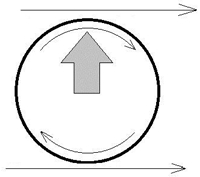
\includegraphics[width=0.25\linewidth]{"./магнус.png"}}
                    %  \includegraphics{"./Q-table.jpg"}
	           \caption{Иллюстрация эффекта Магнуса}
\end{figure}

\subsection{Вывод уравнений и формул}	
Обозначим начальные условия полета мяча:\\
1. Мяч - \textit{абсолютно твёрдое тело}, то есть будем считать, что \textit{взаимное расположение точек мяча не меняется с течением времени}, деформацией во время полета пренебрежем\\
2. Известные параметры мяча: радиус (\textit{\textbf{R}}) и масса (\textit{\textbf{m}})\\
3. Также заданы начальные значения угловой ($\mathbf{\omega_{0}}$) и линейной скоростей ($\mathbf{v_{0}}$)\\
4. Задана некоторая плотность газа - среды, в которой происходит полет мяча ($\mathbf{\rho}$)\\\\

Запишем \textit{закон Ньютона} в общем виде
\begin{equation}
\vec{F} = m \cdot \vec{a}
\end{equation}
Далее распишем силы, действующие на мяч в процессе полета
\begin{equation}
\vec{F}_{\text{тяжести}} + \vec{F}_{\text{Магнуса}}= m \cdot \vec{a}
\end{equation}
Пусть шар находится в потоке набегающего не него идеального газа. Скорость потока на бесконечности $\vec{u}_\infty$. Чтобы сымитировать вращение шара, введем циркуляцию скорости $\Gamma$ вокруг него. Исходя из закона Бернулли, можно получить, что полная сила, действующая в таком случае на шар, равна:
\begin{equation}
\vec{R}= - \rho \vec{\Gamma} \times \vec{u}_\infty \, ,
\end{equation}
где $ \vec{u}_\infty = -\vec{v}$ ($v$ -- линейная скорость мяча);  $\Gamma$ вычислим как
\begin{equation}
\Gamma = \oint \limits^{}_L v_\tau dS \, ,
\end{equation}
$ v_\tau$ -- проекция скорости на касательную к этой кривой, $dS$ -- элемент длины кривой. В случае шара запишем
Запишем формулу для вычисления силы Магнуса в общем виде:
\begin{multline}
\Gamma = \int \limits^R_{-R} 2 \pi \omega (R^2 - x^2) \, dx = 2 \pi \omega \left. \left( R^2x - \frac{x^3}{3}\right)\right|^R_{-R} =\\
=  2 \pi \omega  \left( R^3 - \frac{R^3}{3} +  R^3 - \frac{R^3}{3} \right) = 4 \pi \omega \frac{2 R^3 }{3} = \frac{8 \pi \omega}{3}  R^3  \, ,
\end{multline}
где $R$ -- радиус шара, $\omega$ -- заданная угловая скорость вращения мяча. Будем считать, что вектор угловой скорости задан вдоль 1 оси -- оси $Z$.\\
Тогда запишем формулу для вычисления силы Магнуса:
\begin{equation}
\vec{F}_{\text{Магнуса}} = - \rho \vec{\Gamma} \times \vec{u}_\infty = - \rho  \frac{8 \pi \vec{\omega} }{3}  R^3  \times -\vec{v} = \frac{8 \pi }{3} \rho R^3 \vec{\omega} \times \vec{v}  
\end{equation}

В общем случае будем рассматривать движение мяча в \textit{Декартовой системе координат}, в \textit{трехмерном пространстве}, тогда проекции на оси $X$, $Y$ и $Z$ соотвественно
\begin{equation}
\begin{cases}
 m \ddot{x} =  \frac{8 \pi }{3} \rho R^3 \left( \vec{\omega} \times  \vec{v} \right)_{x} \, ,\\
 m \ddot{y} = \frac{8 \pi }{3} \rho R^3 \left( \vec{\omega} \times  \vec{v} \right)_{y} \, ,\\
 \ddot{z} = g
\end{cases}
\end{equation}


Перейдем к уравнениям для угловой скорости вращения мяча $ \omega $, в частности, найдем выражения для разложения   $ \left( \vec{\omega} \times  \vec{v} \right) $ по единичным векторам, задающим оси координат, $ \vec{i}$, $ \vec{j}$ и $ \vec{k}$
\begin{multline}
\left(  \vec{\omega} \times  \vec{v} \right) = 
\begin{vmatrix}
\vec{i} & \vec{j} & \vec{k} \\
\omega _{x} & \omega _{y} & \omega _{z} \\
v_{x} & v_{y} & v_{z}
\end{vmatrix}
= \vec{i} 
\begin{vmatrix}
\omega _{y} & \omega _{z} \\
v_{y} & v_{z}
\end{vmatrix}
- \vec{j}
\begin{vmatrix}
\omega _{x} & \omega _{z} \\
v_{x} & v_{z}
\end{vmatrix}
+ \vec{k}
\begin{vmatrix}
\omega _{x} & \omega _{y} \\
v_{x} & v_{y}
\end{vmatrix}
=\\
= \vec{i}  \left(\omega _{y} v_{z} -  \omega _{z} v_{y}  \right) + \vec{j} \left( \omega _{z} v_{x} - \omega _{x} v_{z}   \right) + \vec{k} \left( \omega _{x} v_{y} -  \omega _{y} v_{x}   \right) \to \\
\to \left( \vec{\omega} \times  \vec{v}\right)_{x} = \omega _{y} v_{z} -  \omega _{z} v_{y}  =  -  \omega _{z} v_{y}  \\
 \left( \vec{\omega} \times  \vec{v} \right)_{y} = \omega _{z} v_{x} - \omega _{x} v_{z} =  \omega _{z} v_{x}\\
 \left( \vec{\omega} \times  \vec{v} \right)_{z} = \omega _{x} v_{y} -  \omega _{y} v_{x} = 0 \\
\end{multline}
Перейдем к дифференциальному виду уравнений проекций движения мяча на оси координат:
\begin{equation}
\begin{cases}
 m \ddot{x} = - \frac{8 \pi }{3} \rho R^3  \omega _{z} v_{y} \, ,\\
 m \ddot{y} = \frac{8 \pi }{3} \rho R^3 \omega _{z} v_{x} \, ,\\
 \ddot{z} = g
\end{cases}
\end{equation}

Запишем также начальные условия задачи, координаты мяча -- положение его центра масс во времени
\begin{equation}
\begin{cases}
\left(x (0), y(0), z(0) \right)  = \left(0, 0, 0\right)\\
v_{x} (0) = v_{0x}\\
v_{y} (0) = v_{0y}\\
v_{z} (0) = v_{0z}\\
\omega_{x} (0) = 0\\
\omega_{y} (0) = 0\\
\omega_{z} (0) = \omega_{0}
\end{cases}
\end{equation}
\subsection{Решение дифференциальных уравнений}
Для решения соотвествующей системы дифференциальных уравнений был применен \textit{метод Эйлера} численного решения дифференциальных уравнений. Описание метода:\\
\textit{Пусть дана задача Коши для уравнения первого порядка}:
$$ \frac{dy}{dx} = f(x, y), \, \left. y \right|_{x = x_0} = y_0 \, ,$$
\textit{где функция} $f$ \textit{определена на некоторой области} $D \in R^2$. \textit{Решение ищется на полуинтервале} $(x_0, b]$. \textit{На этом промежутке введем узлы} $x_0 < x_1 < ... < x_n \leq b$. \textit{Приближенное решение в узлах} $x_i$, \textit{которое обозначим через} $y_i$,  \textit{определяется по формуле}
$$y_i = y_{i-1} + (x_i - x_{i-1}) f(x_{i-1}, y_{i-1}), \, \, \, i = 1, 2, 3, ..., n.$$
\textit{Эти формулы непосредственно обобщаются на случай систем обыкновенных дифференциальных уравнений.}\\
В данной работе для нахождения численного решения системы линейных однородных уравнений второго порядка метод Эйлера был применен последовательно: сначала для вычисления первой производной, а затем на основе полученного результата -- второй производной.

\subsection{Численный эксперимент. Огибание препятствия заданной ширины}
Молуль силы, действующей на мяч, постоянен, а ее вектор перпендикулярен скорости мяча в любой момент времени и лежит в плоскости $XY$, следовательно, траектория мяча представляет собой фрагмент окружности в плоскости  $XY$. \\
Запишем центростремительное ускорение:
\begin{equation}
a_n = \frac{F}{m} = \frac{8\pi}{3m} \rho \omega v R^3 = \frac{v^2}{r}, \,
\end{equation}
где $r$ -- радиус кривизны дуги, по которой движется мяч. Тогда
\begin{equation}
\frac{v}{\omega} =  \frac{8\pi}{3m} \rho r R^3 \to \omega (v) = \frac{v}{k}, \, k =  \frac{8\pi}{3m} \rho r R^3
\end{equation}
Пусть линейная скорость задана вдоль оси $X$, а препятствие представляет собой бесконечный цилиндр.\\
На основе геометрической модели (рисунок ?) составим выражения:
\begin{equation}
|Y_0| - R_{\text{пр}} = O'B 
\end{equation}
\begin{equation}
O'B = \sqrt{\left( Y_0 - Y_{\text{пр}} \right)^2 + X_{\text{пр}}^2} 
\end{equation}
Откуда выразим $Y_0$ -- радиус траектории мяча при касании препятствия:
\begin{equation}
Y_0 = \frac{X_{\text{пр}}^2 +  Y_{\text{пр}}^2 - R_{\text{пр}}^2 }{2 \left(  Y_{\text{пр}} - R_{\text{пр}} \right) \frac{\sqrt{ Y_{\text{пр}}^2}}{ Y_{\text{пр}}}}
\end{equation}
Пусть $h$ -- коэффициент отношения расстояния от центра координат до пересечения прямой, на которой лежит центр координат и центр препятствия, и траектории мяча к расстоянию от начала координат до центра препятствия.
\begin{equation}
OO' = \sqrt{ X_{\text{пр}}^2 + Y_{\text{пр}}^2}
\end{equation}
\begin{equation}
BC^2 = \left( X_{\text{пр}} h \right)^2 + \left( Y_0 - Y_{\text{пр}} h \right)^2
\end{equation}
\begin{equation}
BC^2 =  Y_0^2
\end{equation}
\begin{equation}
h = \frac{2 Y_0  Y_{\text{пр}}}{X_{\text{пр}}^2 +  Y_{\text{пр}}^2 }
\end{equation}
\begin{equation}
\phi = 2 \alpha, 
\end{equation}
где $\phi = \angle OBC$, $\alpha = \angle OBK$
\begin{equation}
\sin \alpha = \frac{OO' h}{2 Y_0}
\end{equation}
\begin{equation}
\phi = 2 \arcsin \alpha
\end{equation}
Пусть $S$ -- длина траектории до пересечения объектом прямой, соединяющей центр координат и центр препятствия.

\begin{equation}
S = \phi Y_0 =  Y_0  2 \arcsin \alpha =  Y_0  2 \arcsin \frac{ \sqrt{ X_{\text{пр}}^2 + Y_{\text{пр}}^2} h}{2 Y_0}
\end{equation}
Мяч находится в поле тяжести, по оси $Z$ ускорение равно $g$, соотвественно, время полета $t = 2 \frac{v_z}{g}$, $v_z$ -- начальная скорость по вертикали.\\
Найдем угловую скорость, для которой выполняется нужное соотношение с минимальной линейной скоростью мяча, при которой он сможет преодолеть необходимое расстояние.\\
В качестве результата проводится анализ графика (Рисунок ?), демонстрирующего поведение системы при заданных угловой и линейной скоростях.
\begin{figure}[!h]
		\center{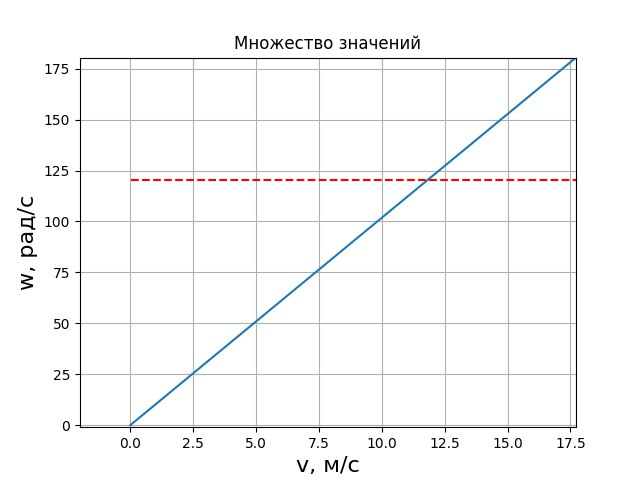
\includegraphics[width=0.75\linewidth]{"./graphics/don_th.jpg"}}
                    %  \includegraphics{"./Q-table.jpg"}
	           \caption{Множество значений скоростей}
\end{figure}
При нахождении левее пунктирной линии, тогда мячу не хватает времени полета для того, чтобы обогнуть препятствие, справа от пунктирной линии и ниже сплошной линии -- обогнуть препятствие не удастся, если выше -- мяч обогнул препятствие. Расположение на сплошной линии -- касание препятствия при полете.\\
Рассчитанные значения соотвествуют координатам точки пересечения сплошной и пунктирной линий.




\section{Моделирование процесса}
\subsection{Общие сведения}
Исходные данные программы:\\
1. Масса мяча (по футбольным стандартам) \textbf{m = 0.430 кг}\\
2. Радиус мяча (при длине окружности около 70 см)  \textbf{R = 0.11 м}\\
3. Плотность воздуха (при $T = 15 C^{\text{o}}$) $\rho = 1.225 \frac{\text{кг}}{\text{м}^3}$\\
4. Координаты начальной точки запуска мяча $(0, 0, 0)$\\\\
Данные вводимые пользователем:\\
1. Проекции линейной скорости на оси $x, y, z$, \textit{ограничение: }  $v_{z_{0}} > 0$\\
2. Значение угловой скорости $\omega$, \textit{ примечание: по умолчанию вектор угловой скорости направлен вдось оси z }\\
3*. Задание ширины препятствия\\\\
Выходные данные:\\
1. Для первой части эксперимента с заданными линейной и угловой скоростями выводится графическое представление полета на плоскости $xy$\\
2. Для эксперимента с заданным препятствием выводятся подходящие значения угловой и линейных скоростей, которые необходимо задать, чтобы обойти препятствие\\


\subsection{Результаты работы программы}
Программа написана на языке \textit{Python 3} с использованием библиотеки \textit{Matplotlib}. \\
Ниже представлены графики различных проекций траектории полета футбольного мяча при разных заданных значениях угловой скорости $\omega$ и одинаковых значениях линейной скорости.\\
Для $\omega = 30, 10, 0  \text{ рад/с} $:
\begin{figure}[!h]
		\center{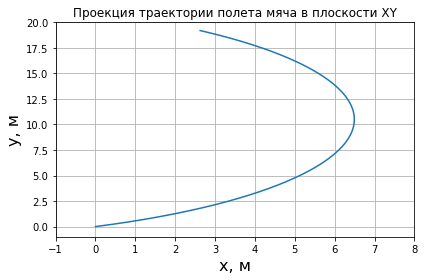
\includegraphics[width=0.75\linewidth]{"./graphics/xy_10_5_10_30.png"}}
                    %  \includegraphics{"./Q-table.jpg"}
	           \caption{При $v_x = 10 \text{ м/с}, \, v_y = 5  \text{ м/с}, \, v_z = 10  \text{ м/с}, \, \omega = 30 \text{ рад/с}$ пр. $XY$}
\end{figure}

\begin{figure}[!h]
		\center{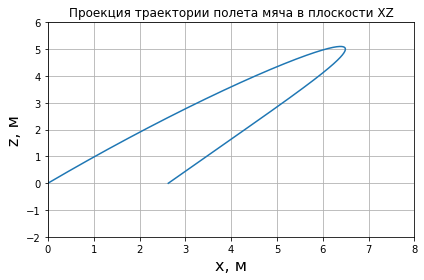
\includegraphics[width=0.75\linewidth]{"./graphics/xz_10_5_10_30.png"}}
                    %  \includegraphics{"./Q-table.jpg"}
	           \caption{При $v_x = 10 \text{ м/с}, \, v_y = 5  \text{ м/с}, \, v_z = 10  \text{ м/с}, \, \omega = 30 \text{ рад/с}$ пр. $XZ$}
\end{figure}

\begin{figure}[!h]
		\center{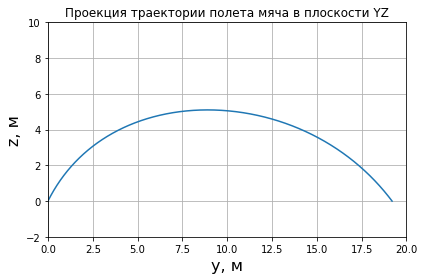
\includegraphics[width=0.75\linewidth]{"./graphics/yz_10_5_10_30.png"}}
                    %  \includegraphics{"./Q-table.jpg"}
	           \caption{При $v_x = 10 \text{ м/с}, \, v_y = 5  \text{ м/с}, \, v_z = 10  \text{ м/с}, \, \omega = 30 \text{ рад/с}$ пр. $YZ$}
\end{figure}

\begin{figure}[!h]
		\center{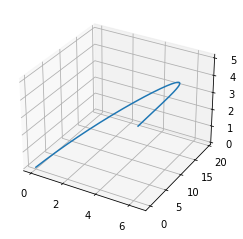
\includegraphics[width=0.75\linewidth]{"./graphics/xyz_10_5_10_30.png"}}
                    %  \includegraphics{"./Q-table.jpg"}
	           \caption{При $v_x = 10 \text{ м/с}, \, v_y = 5  \text{ м/с}, \, v_z = 10  \text{ м/с}, \, \omega = 30 \text{ рад/с}$ пр. $XYZ$}
\end{figure}

\newpage
\begin{figure}[!h]
		\center{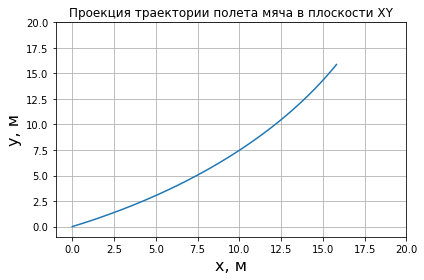
\includegraphics[width=0.75\linewidth]{"./graphics/xy_10_5_10_10.png"}}
                    %  \includegraphics{"./Q-table.jpg"}
	           \caption{При $v_x = 10 \text{ м/с}, \, v_y = 5  \text{ м/с}, \, v_z = 10  \text{ м/с}, \, \omega = 10 \text{ рад/с}$ пр. $XY$}
\end{figure}

\begin{figure}[h]
		\center{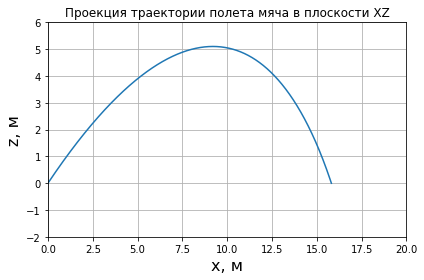
\includegraphics[width=0.75\linewidth]{"./graphics/xz_10_5_10_10.png"}}
                    %  \includegraphics{"./Q-table.jpg"}
	           \caption{При $v_x = 10 \text{ м/с}, \, v_y = 5  \text{ м/с}, \, v_z = 10  \text{ м/с}, \, \omega = 10 \text{ рад/с}$ пр. $XZ$}
\end{figure}

\begin{figure}[h]
		\center{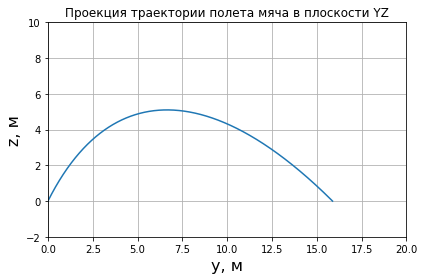
\includegraphics[width=0.75\linewidth]{"./graphics/yz_10_5_10_10.png"}}
                    %  \includegraphics{"./Q-table.jpg"}
	           \caption{При $v_x = 10 \text{ м/с}, \, v_y = 5  \text{ м/с}, \, v_z = 10  \text{ м/с}, \, \omega = 10 \text{ рад/с}$ пр. $YZ$}
\end{figure}

\begin{figure}[h]
		\center{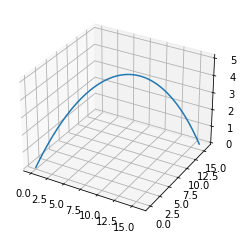
\includegraphics[width=0.75\linewidth]{"./graphics/xyz_10_5_10_10.png"}}
                    %  \includegraphics{"./Q-table.jpg"}
	           \caption{При $v_x = 10 \text{ м/с}, \, v_y = 5  \text{ м/с}, \, v_z = 10  \text{ м/с}, \, \omega = 10 \text{ рад/с}$ пр. $XYZ$}
\end{figure}

\newpage
\begin{figure}[!h]
		\center{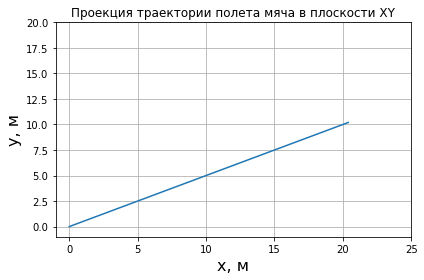
\includegraphics[width=0.75\linewidth]{"./graphics/xy_10_5_10_0.png"}}
                    %  \includegraphics{"./Q-table.jpg"}
	           \caption{При $v_x = 10 \text{ м/с}, \, v_y = 5  \text{ м/с}, \, v_z = 10  \text{ м/с}, \, \omega = 0 \text{ рад/с}$ пр. $XY$}
\end{figure}

\begin{figure}[h]
		\center{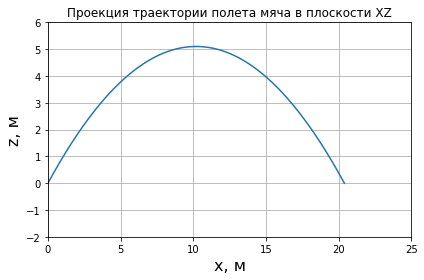
\includegraphics[width=0.75\linewidth]{"./graphics/xz_10_5_10_0.png"}}
                    %  \includegraphics{"./Q-table.jpg"}
	           \caption{При $v_x = 10 \text{ м/с}, \, v_y = 5  \text{ м/с}, \, v_z = 10  \text{ м/с}, \, \omega = 0 \text{ рад/с}$ пр. $XZ$}
\end{figure}

\begin{figure}[h]
		\center{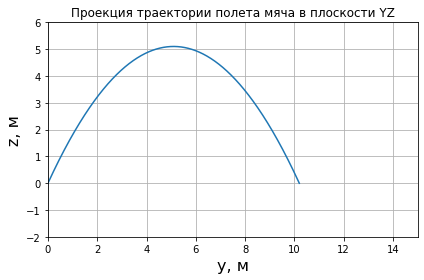
\includegraphics[width=0.75\linewidth]{"./graphics/yz_10_5_10_0.png"}}
                    %  \includegraphics{"./Q-table.jpg"}
	           \caption{При $v_x = 10 \text{ м/с}, \, v_y = 5  \text{ м/с}, \, v_z = 10  \text{ м/с}, \, \omega = 0 \text{ рад/с}$ пр. $YZ$}
\end{figure}

\begin{figure}[h]
		\center{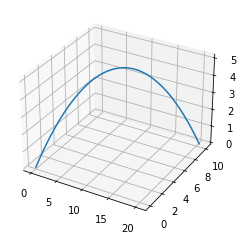
\includegraphics[width=0.75\linewidth]{"./graphics/xyz_10_5_10_0.png"}}
                    %  \includegraphics{"./Q-table.jpg"}
	           \caption{При $v_x = 10 \text{ м/с}, \, v_y = 5  \text{ м/с}, \, v_z = 10  \text{ м/с}, \, \omega = 0 \text{ рад/с}$ пр. $XYZ$}
\end{figure}


\end{document}













